
\subsection{Bi-level optimisation}
\label{sec-oopt}

The ``classical'' tuning problem can be
    \begin{itemize}
        \item Incompatible datasets and mismodelling in MC generator necessitate introduction of tuning weights $w_b$
        \item Adjusting the weights has so far been a manual procedure
        \item The user would iteratively run the ``inner optimisation`` and look at resulting plots
        \item We propose an automated procedure for this ''outer optimisation``:
            \begin{itemize}
                \item Write goodness-of-fit in terms of histograms/observables
                \item The parameter space is now the observable-weight space
                \item Inner optimisation yields best fit point, \phat, for given $$\left\{w_\mathcal{O}\right\}$$
                \item \phat is used to evaluate an objective function for the outer optimisation
            \end{itemize}
    \end{itemize}
$$
    \phisq(\p|\left\{w_\mathcal{O}\right\}) =
    \sum_{\mathcal{O}=1}^N w_\mathcal{O}^2 \cdot
    \sum_{b\in \mathcal{O}}
  \frac{ (f_b(\p) - \mathcal{R}_b)^2 }{   \Delta^2}
$$

    \begin{itemize}
        \item For given \phat, we can calculate the per-observable goodness-of fit
    \end{itemize}
$$
    \nu_\mathcal{O}(\phato) =
    \frac{1}{N_\text{bins}(\mathcal{O})}
    \sum_{b\in \mathcal{O}}
  \frac{ (f_b(\phato) - \mathcal{R}_b)^2 }{  \Delta^2}, \ {\cal O} =1,\ldots, N
$$
\begin{itemize}
    \item With $N$ such measures, we can calculate mean and standard deviation
\end{itemize}
$$%\begin{equation} 
 \mu(w_{\cal O}, \p^*) = \frac{1}{N}\sum_{{\cal O}=1}^N \nu_{\cal O}(w_{\cal O}, \p^*)
$$%\end{equation}	
$$% \begin{equation} 
 \sigma^2(w_{\cal O}, \p^*) = \frac{1}{N}\sum_{{\cal O}=1}^N \left[\nu_{\cal O}(w_{\cal O}, \p^*) -\mu(w_{\cal O}, \p^*)\right]^2
$$%\end{equation}	
    \begin{itemize}
            \item And construct an objective function to minimise
        \end{itemize}
$$% \begin{equation}
\min_{w_{\cal O}\in[0,1]} \lambda \mu(w_{\cal O}, \p^*) + \sigma^2(w_{\cal O}, \p^*),\quad \text{s.t. } \sum_{{\cal O}=1}^N w_{\cal O} =1.
$$%\end{equation}	


    \begin{itemize}
        \item Minimisation of portfolio objective is iterative
        \item We train a radial basis function and use it to walk through the weight space
        \item Convergence is fast but depends on initial guess $\to$ multi-start approach (that's ok since inner optimisation is really fast)
    \end{itemize}
    \begin{minipage}{.48\textwidth}%
        \begin{center}
            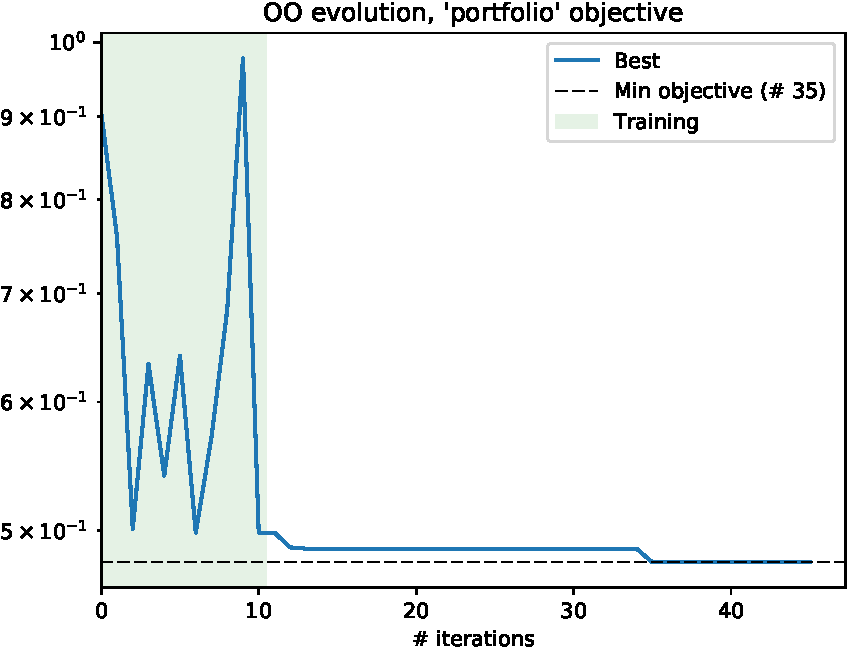
\includegraphics[width=.98\textwidth]{oo/chain-3-report.pdf}
        \end{center}
    \end{minipage}%
    \begin{minipage}{.04\textwidth}%
    \end{minipage}%
    \begin{minipage}{.48\textwidth}%
        \begin{center}
            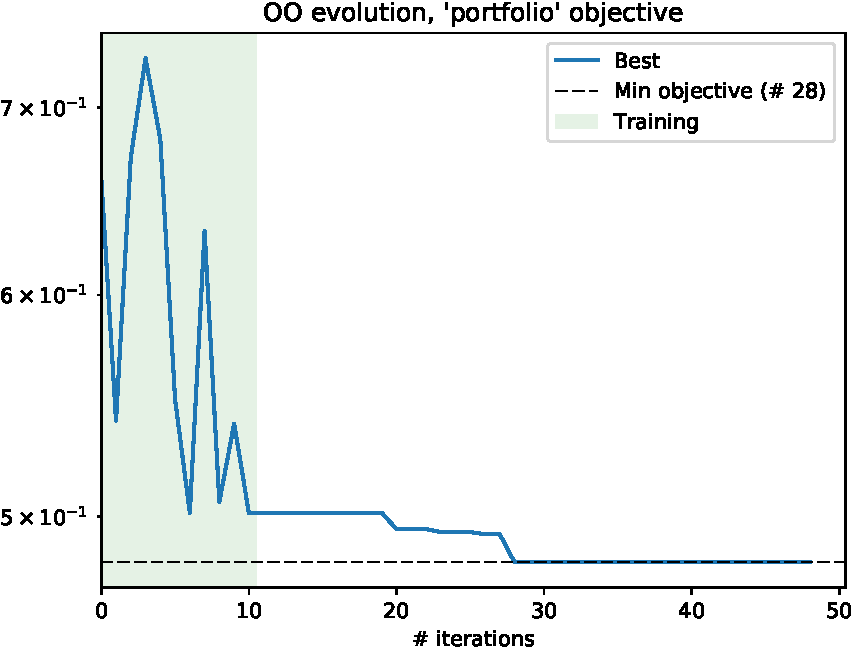
\includegraphics[width=.98\textwidth]{oo/chain-1-report.pdf}
        \end{center}
    \end{minipage}%

%\begin{frame}{}
    %\begin{center}
        %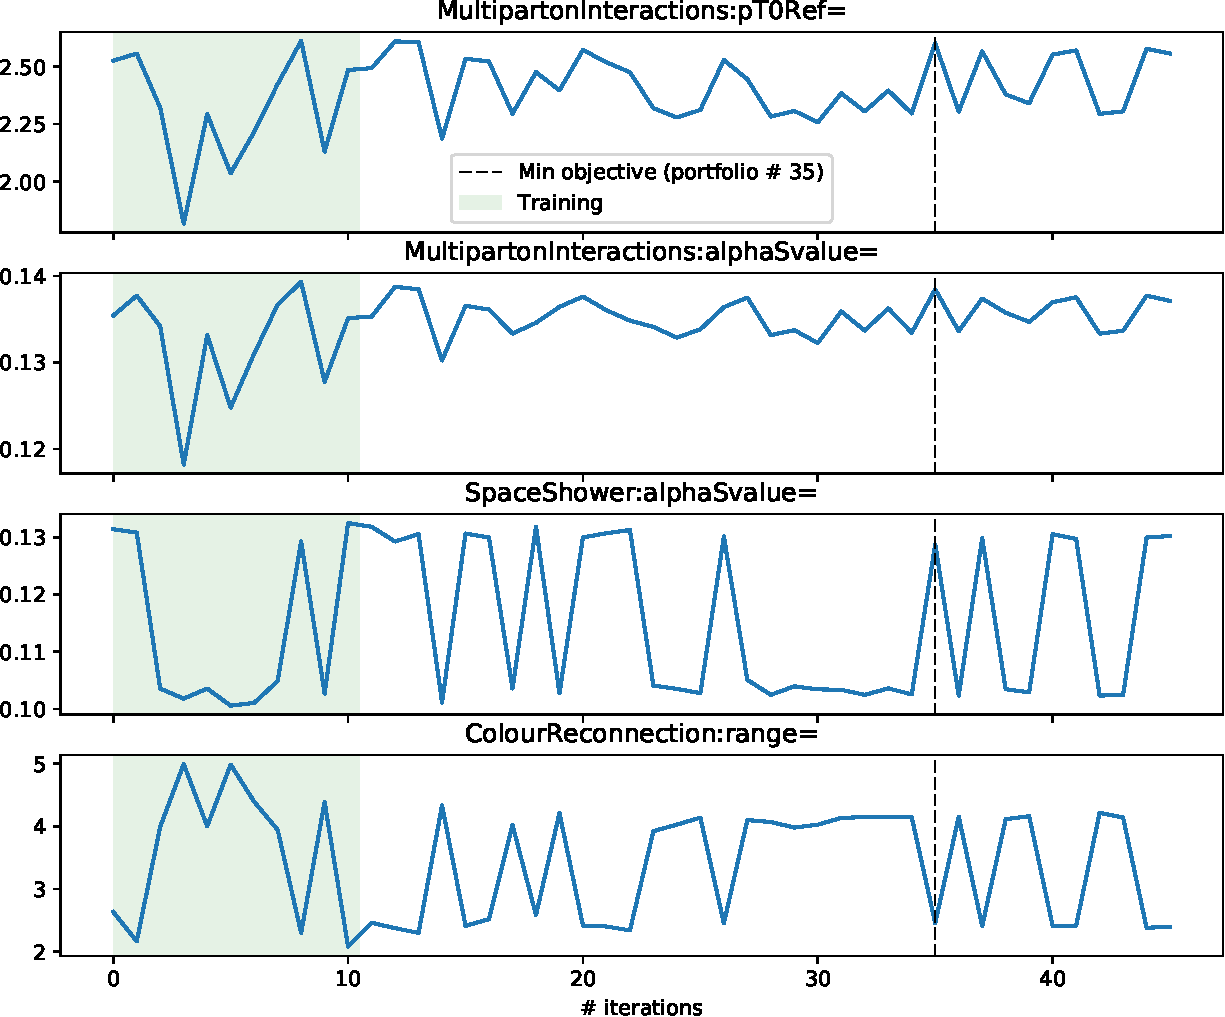
\includegraphics[width=.98\textwidth]{oo/chain-3-report-pevolution.pdf}
    %\end{center}
%\end{frame}
\begin{frame}{Evolution of weights}
    \begin{itemize}
        \item This plot shows the $\left\{w_\mathcal{O}\right\}$  of the outer optimisation
        \item Controlplot to check that weight space is reasonably sampled
    \end{itemize}
    \begin{center}
        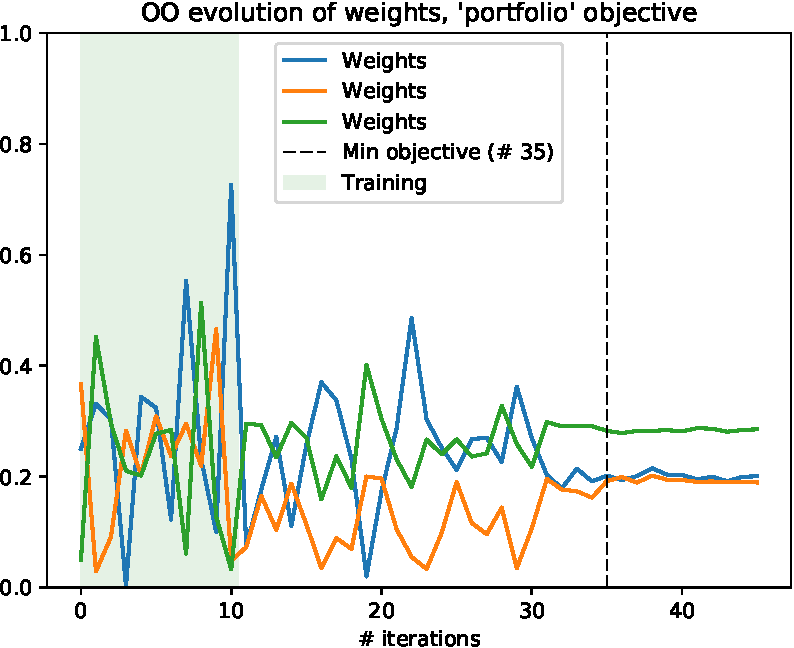
\includegraphics[width=.78\textwidth]{oo/chain-3-report-wevolution.pdf}
    \end{center}
\end{frame}

\begin{frame}{Evolution of inner optimisation}
    \begin{itemize}
        \item This plot shows the \phat of the inner optimisation
        \item Shows the correlation of parameters
    \end{itemize}
    \begin{center}
        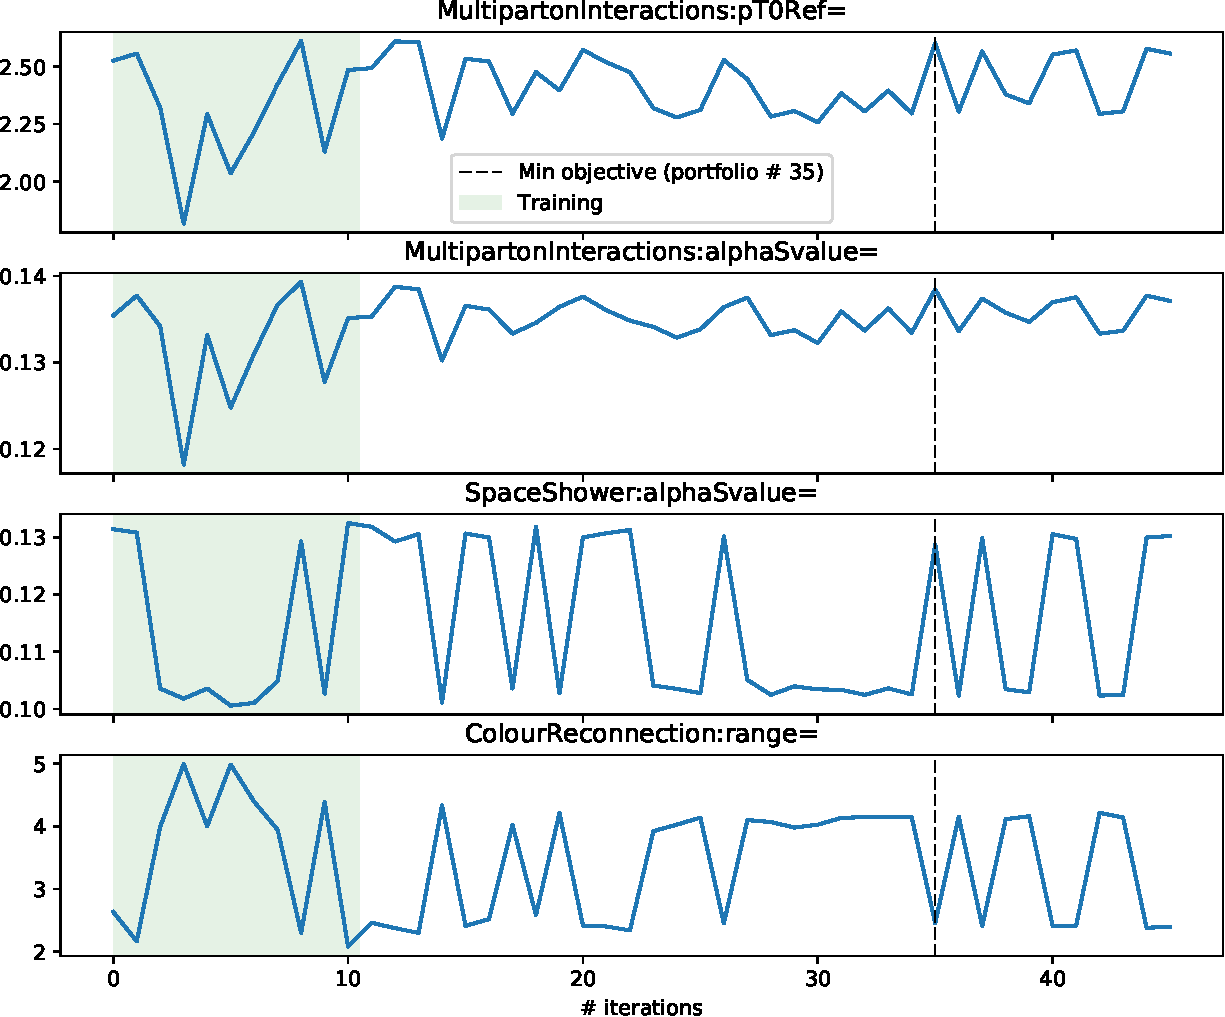
\includegraphics[width=.78\textwidth]{oo/chain-3-report-pevolution.pdf}
    \end{center}
\end{frame}

\begin{frame}{Comparison of results}
    \begin{minipage}{.48\textwidth}%
        \begin{center}
            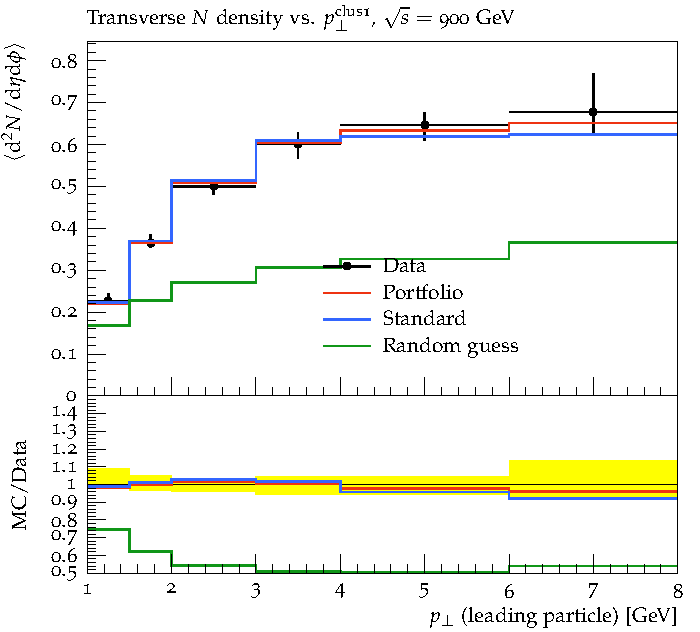
\includegraphics[width=.92\textwidth]{oo/test_cmp_1_std/ATLAS_2011_S8994773/d01-x01-y01.pdf}\\
            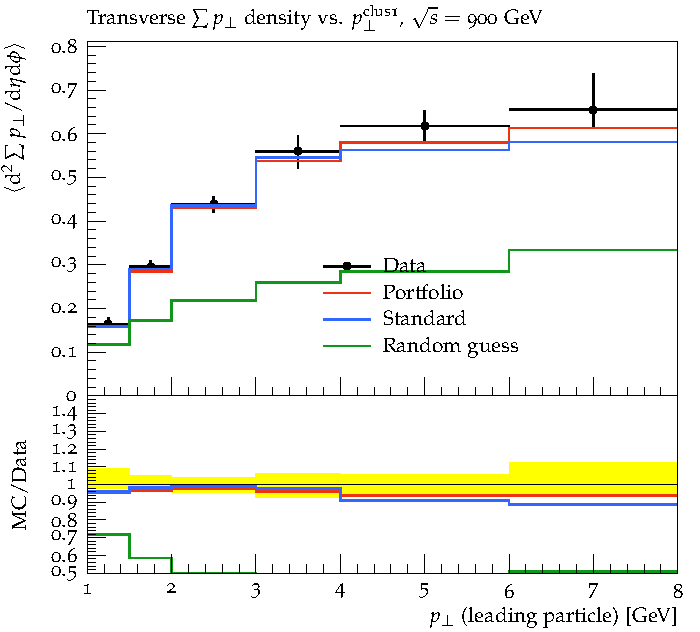
\includegraphics[width=.92\textwidth]{oo/test_cmp_1_std/ATLAS_2011_S8994773/d03-x01-y01.pdf}
        \end{center}
    \end{minipage}%
    \begin{minipage}{.04\textwidth}%
    \end{minipage}%
    \begin{minipage}{.48\textwidth}%
        \begin{center}
            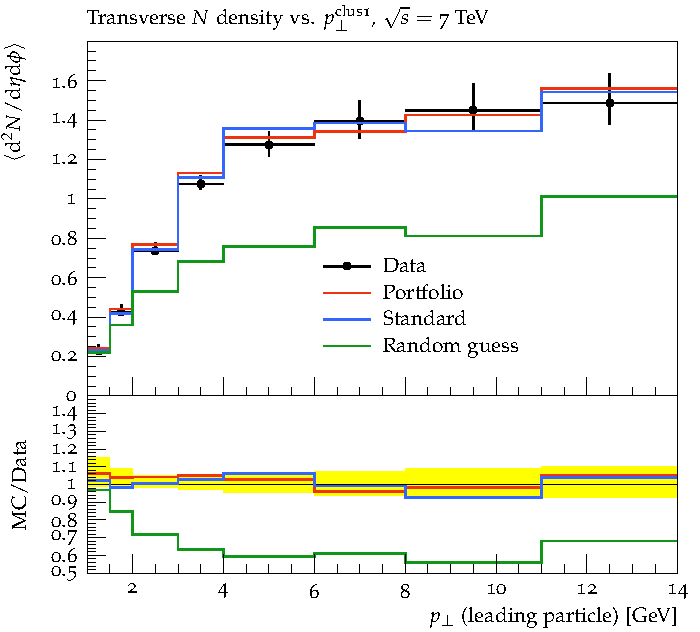
\includegraphics[width=.92\textwidth]{oo/test_cmp_1_std/ATLAS_2011_S8994773/d02-x01-y01.pdf}\\
            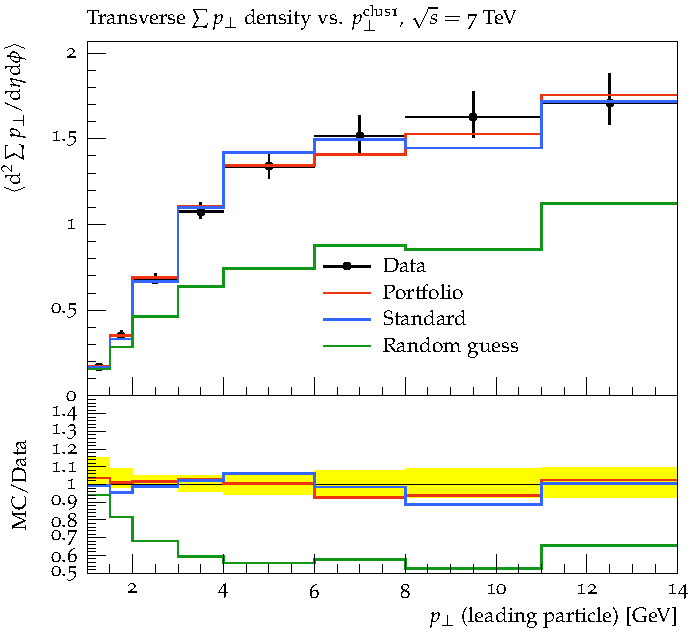
\includegraphics[width=.92\textwidth]{oo/test_cmp_1_std/ATLAS_2011_S8994773/d04-x01-y01.pdf}
        \end{center}
    \end{minipage}%
\end{frame}
